% Options for packages loaded elsewhere
\PassOptionsToPackage{unicode}{hyperref}
\PassOptionsToPackage{hyphens}{url}
\PassOptionsToPackage{dvipsnames,svgnames,x11names}{xcolor}
%
\documentclass[
  12pt,
]{article}
\usepackage{amsmath,amssymb}
\usepackage{lmodern}
\usepackage{iftex}
\ifPDFTeX
  \usepackage[T1]{fontenc}
  \usepackage[utf8]{inputenc}
  \usepackage{textcomp} % provide euro and other symbols
\else % if luatex or xetex
  \usepackage{unicode-math}
  \defaultfontfeatures{Scale=MatchLowercase}
  \defaultfontfeatures[\rmfamily]{Ligatures=TeX,Scale=1}
\fi
% Use upquote if available, for straight quotes in verbatim environments
\IfFileExists{upquote.sty}{\usepackage{upquote}}{}
\IfFileExists{microtype.sty}{% use microtype if available
  \usepackage[]{microtype}
  \UseMicrotypeSet[protrusion]{basicmath} % disable protrusion for tt fonts
}{}
\usepackage{xcolor}
\usepackage[margin=1in]{geometry}
\usepackage{graphicx}
\makeatletter
\def\maxwidth{\ifdim\Gin@nat@width>\linewidth\linewidth\else\Gin@nat@width\fi}
\def\maxheight{\ifdim\Gin@nat@height>\textheight\textheight\else\Gin@nat@height\fi}
\makeatother
% Scale images if necessary, so that they will not overflow the page
% margins by default, and it is still possible to overwrite the defaults
% using explicit options in \includegraphics[width, height, ...]{}
\setkeys{Gin}{width=\maxwidth,height=\maxheight,keepaspectratio}
% Set default figure placement to htbp
\makeatletter
\def\fps@figure{htbp}
\makeatother
\setlength{\emergencystretch}{3em} % prevent overfull lines
\providecommand{\tightlist}{%
  \setlength{\itemsep}{0pt}\setlength{\parskip}{0pt}}
\setcounter{secnumdepth}{5}
\newlength{\cslhangindent}
\setlength{\cslhangindent}{1.5em}
\newlength{\csllabelwidth}
\setlength{\csllabelwidth}{3em}
\newlength{\cslentryspacingunit} % times entry-spacing
\setlength{\cslentryspacingunit}{\parskip}
\newenvironment{CSLReferences}[2] % #1 hanging-ident, #2 entry spacing
 {% don't indent paragraphs
  \setlength{\parindent}{0pt}
  % turn on hanging indent if param 1 is 1
  \ifodd #1
  \let\oldpar\par
  \def\par{\hangindent=\cslhangindent\oldpar}
  \fi
  % set entry spacing
  \setlength{\parskip}{#2\cslentryspacingunit}
 }%
 {}
\usepackage{calc}
\newcommand{\CSLBlock}[1]{#1\hfill\break}
\newcommand{\CSLLeftMargin}[1]{\parbox[t]{\csllabelwidth}{#1}}
\newcommand{\CSLRightInline}[1]{\parbox[t]{\linewidth - \csllabelwidth}{#1}\break}
\newcommand{\CSLIndent}[1]{\hspace{\cslhangindent}#1}
\usepackage{setspace} \setstretch{1.15} \usepackage{float} \floatplacement{figure}{t} \usepackage[labelsep=period]{caption}
\usepackage{booktabs}
\usepackage{longtable}
\usepackage{array}
\usepackage{multirow}
\usepackage{wrapfig}
\usepackage{float}
\usepackage{colortbl}
\usepackage{pdflscape}
\usepackage{tabu}
\usepackage{threeparttable}
\usepackage{threeparttablex}
\usepackage[normalem]{ulem}
\usepackage{makecell}
\usepackage{xcolor}
\ifLuaTeX
  \usepackage{selnolig}  % disable illegal ligatures
\fi
\IfFileExists{bookmark.sty}{\usepackage{bookmark}}{\usepackage{hyperref}}
\IfFileExists{xurl.sty}{\usepackage{xurl}}{} % add URL line breaks if available
\urlstyle{same} % disable monospaced font for URLs
\hypersetup{
  pdftitle={Simulations of fold number selection in cross-validation of linear and LASSO regression},
  pdfauthor={Angelos Vasilopoulos; Gregory J. Matthews},
  colorlinks=true,
  linkcolor={cyan},
  filecolor={Maroon},
  citecolor={Blue},
  urlcolor={cyan},
  pdfcreator={LaTeX via pandoc}}

\title{Simulations of fold number selection in cross-validation of
linear and LASSO regression}
\author{Angelos Vasilopoulos \and Gregory J. Matthews}
\date{}

\begin{document}
\maketitle
\begin{abstract}
\emph{k}-fold cross-validation is a popular method of error estimation
for model selection in computational research. However, there is limited
focus in the literature on the question of what fold number \emph{k} is
appropriate for various dataset dimensions. Here we review relevant
literature and present a simulation of linear and least absolute
shrinkage and selection operator (LASSO) regression prediction error
estimation at various values of \emph{k} and sample size \emph{n}. In
agreement with a growing body of literature, we find that contrary to a
persisting understanding, there is no bias-variance trade-off in
selection of \emph{k}. Instead, with increasing \emph{k} both bias and
variance decrease, perhaps asymptotically. Our results also suggest a
predictable relationship between optimal values of \emph{k} and
\emph{n}. \textbar{} \emph{Keywords}: cross-validation, optimization,
fold number
\end{abstract}

\hypertarget{sec:intro}{%
\section{Introduction}\label{sec:intro}}

\(k\)-fold cross-validation is a popular method of error estimation for
model selection in computational research. \(n\) observations are
divided into \(k\) groups. In a first iteration, \(i = k - 1\) groups
are used as a training set. The remaining group is used as a test set to
calculate estimated prediction error (\(\mathrm{\widehat{PE}}\)). This
process is repeated \(i\) times, with a different test set in each
iteration. The average of \(k\) estimates of \(\mathrm{PE}\)
\[\hat{\theta} = CV_{(k)} = \frac{1}{k}\sum_{i=1}^{k}\mathrm{\widehat{PE}}_i\]
is meant to estimate the true model error \(\theta\), i.e., the error of
the model tested on the population.

Despite the popularity of cross-validation, there is limited focus in
the literature on the question of what fold number \(k\) is appropriate
for cross-validation with a dataset of a given size. One popular idea is
that selection of \(k\) comes with a bias-variance
trade-off---specifically, that as \(k\) increases, the bias
\(Bias(\hat{\theta}) = \mathrm{E}(\hat{\theta}) - \theta\) and variance
\(Var(\hat{\theta}) = \mathrm{E}(\hat{\theta}^2) - \mathrm{E}(\hat{\theta})^2\)
of \(k\)-fold error estimation decrease and increase, respectively. This
idea appears in early literature (Efron
(\protect\hyperlink{ref-Efron1983}{1983}); Kohavi
(\protect\hyperlink{ref-Kohavi2001}{2001})) but also in modern, widely
used textbooks (James et al. (\protect\hyperlink{ref-James2021}{2021})).

Subsequent, albeit limited, literature argues differently. In the case
of leave-one-out cross-validation (LOOCV), i.e., with \(k = n\), some
authors suggest that asymptotically both bias and variance of error
estimation decrease as \(k\) increases (Burman
(\protect\hyperlink{ref-Burman1989}{1989})) and that bias and variance
of error estimation are uniformly low (Breiman and Spector
(\protect\hyperlink{ref-Breiman1992}{1992})).

More recently have been proposed ways to quantify the variance reduction
achieved by cross-validation when the true prediction error
(\(\mathrm{PE}\)) is not known, e.g., as mean-square stability (Kale,
Kumar, and Vassilvitskii (\protect\hyperlink{ref-Kale2011}{2011})),
where
\[\underset{S,z,z'}{\mathrm{E}}[(\ell_{\mathcal A(S)}(z) - \ell_{\mathcal A(S^{i,z'})}(z))^2] \le \beta,\]
i.e., the expectation of the squared difference in loss \(\ell\) of an
algorithm \(\mathcal A\) over a dataset \(S\) and over a dataset \(S'\)
such that one element \(z' \sim Z\) has been added to \(S\) is less than
\(\beta\), which depends on the algorithm; or as loss stability (Kumar
et al. (\protect\hyperlink{ref-Kumar2013}{2013})), where
\[\underset{S,z,z'}{\mathrm{E}}[(\ell'_{\mathcal A(S)}(z) - \ell'_{\mathcal A(S^{i,z'})}(z))^2] \le \gamma,\]
\(\ell'_{\mathcal A(S)}(z) = \ell_{\mathcal A(S)}(z) - \bar{\ell}_{\mathcal A(S)}(z)\),
and \(\gamma\) depends on the algorithm. However, it has also been
demonstrated that, due to overlap between training and test sets in
cross-validation, there is no universal (i.e., valid under all
distributions) unbiased estimator of the variance of \(k\)-fold
cross-validation (Bengio and Grandvalet
(\protect\hyperlink{ref-Bengio2004}{2004})).

In addition to theoretical analyses of variance reduction by
cross-validation, there are some simulation results showing this
phenomenon. However, simulations currently in the literature provide
limited insight into the dependence of optimal fold number
\(k_\mathrm{optimal}\) on sample size \(n\) (Zhang and Yang
(\protect\hyperlink{ref-Zhang2015}{2015})) or involve biased variance
calculations (Marcot and Hanea
(\protect\hyperlink{ref-Marcot2021}{2021})). Here we present a
simulation of linear regression and least absolute shrinkage and
selection operator (LASSO) regression to observe the relationship of
cross-validation fold number \(k\) to model selection accuracy for
various samples of size \(n\) of a known population.

\hypertarget{simulation}{%
\section{Simulation}\label{simulation}}

Consider a population of size N = 500,000 with five of \(P = 100\)
features \(X_1...X_{100} \sim N(0, 1)\) a linear combination of feature
\(Y = \beta_0 + \beta_1X_1 + \cdots + \beta_5X_5 + \epsilon\) where
\(\beta_1 = \cdots = \beta_5 = 1\) and \(\epsilon \sim N(0, 10)\). The
true model of \(Y\) is \(f \in F\), a set of competing models.
\(f = \mathrm{E}(Y) = \beta_0 + \beta_1X_1 + \cdots + \beta_5X_5\) and
its mean squared error (\(\mathrm{MSE}\)) is
\[\theta = \mathrm{MSE}[\mathrm{E}(Y)] = \frac{\sum_{i=1}^{N}[Y_i - \mathrm{E}(Y_i)]^2}{N}.\]

From the population we take a sample of size \(n\). We estimate \(Y\) as
\(\hat{Y}\) by regression on a subset of \(X_1...X_{100}\), regression
coefficients estimated by the least squares method, and compute
\(\mathrm{MSE}(\hat{Y})\) by \(k\)-fold cross-validation as
\[\hat{\theta} = \mathrm{MSE}(\hat{Y}) = \frac{1}{k}\sum_{j=1}^{k}\frac{\sum_{i=1}^{n/k}(Y_{j_i} - \hat{Y_{j_i}})^2}{n/k}\]
where \(j_i\) is the index of the \(i^{th}\) element of the \(j^{th}\)
fold.

In addition to regression with \(X_1...X_5\), \(f\), we under-fit with
\(X_1...X_3\), over-fit with \(X_1...X_{20}\) and \(X_1...X_{100}\), and
do regression with noise \(X_6...X_{100}\) only, for each \(k \in\) \{2,
10, 20, 30, \ldots, \(n\)\} for each \(n \in\) \{100, 200, 300, \ldots,
1000\}. We perform this simulation 1000 times and then calculate
simulation-wise \(\mathrm{MSE}(\hat{\theta})\) for each \(k\), for each
\(n\).

We perform an additional 1000 simulations predicting \(Y\) as
\(\hat{Y}\) by LASSO regression instead of linear regression for each
\(k \in\) \{2, 10, 20, 30, \ldots, 100, \(n\)\} for each \(n \in\)
\{250, 500, 750, 1000\}. To avoid data leakage, we introduce an inner
5-fold cross-validation loop for the selection of parameter \(\lambda\)
as in the minimization of
\[\sum_{i=j}^{p}(Y_j - \beta_j)^2 + \lambda\sum_{j=1}^{p}|\beta_j|.\]

For each \(k\), for each \(n\), we count the number of times \(A\) that
the true model is selected and consider as optimal fold number for each
\(n\) the value \(k_\mathrm{optimal}\), at which \(A\) is the highest.

This is because in practice the model with the lowest
\(\mathrm{\widehat{PE}}\) is more likely to be selected. We refer to
this as lowest-error model selection. As our simulation results show,
however, it is possible for \(k\)-fold cross-validation to result in
calculations of \(\mathrm{MSE}(\hat{\theta})\) such that a competing
model \(\hat{f}\) has a lower \(\mathrm{\widehat{PE}}\) than the true
model \(f\). This false model may have the lowest
\(\mathrm{\widehat{PE}}\) but its generalization error will be higher in
the long-run (i.e., when tested on a large part of the population) than
the generalization error of the true model. Thus, it is preferable for
the value of \(k\) selected to result in \(f\) having the lowest
\(\mathrm{\widehat{PE}}\).

Having considered the effect of \(k\) on model selection accuracy for a
given \(n\), we may also consider the relationship of
\(k_\mathrm{optimal}\) and \(n\). Our results suggest that after a
certain value of \(k\), changes in \(A\) become negligible, in the case
of linear regression, or negative, in the case of LASSO regression, and
resource-expensive increases of fold number become undesirable. We refer
to this ``point of diminishing returns'' as \(k_\mathrm{optimal}^*\).

To estimate \(k_\mathrm{optimal}*\) for each \(n\), we first fit to the
dataset \((k,A)\) for each sample size \(n\) a non-linear least squares
model of the form \[\hat{A}(k) = Bk + C + Dk^{-1} + Ek^{-2}\] with
constants \(B\) to \(E\) specific to each \(n\) and constants \(B\) and
\(E\) set to zero for linear regression. We then draw a line \(L\)
through \((k_1, \hat{A}_1)\) and \((k_n, \hat{A}_n)\) and maximize the
perpendicular distance \(d\) of each point on \(\hat{A}\) from \(L\), so
that \[k_\mathrm{optimal}^* = {\arg\max}_k{d[\hat{A}(k)-L]}.\]

\hypertarget{results-and-discussion}{%
\section{Results and discussion}\label{results-and-discussion}}

Interpretations of early literature have resulted in lasting
misconceptions about the use of cross-validation. Such misconceptions
include the idea that there is a bias-variance trade-off
\(Bias^2(\hat{\theta}) \propto 1/Var(\hat{\theta})\) associated with
selection of \(k\) and that \(k = 10\) is the best value to use in
\(k\)-fold cross-validation (Kohavi
(\protect\hyperlink{ref-Kohavi2001}{2001})).

In agreement with a small but growing body of literature, our simulation
results suggest that neither of these ideas are necessarily correct.
Instead, in the context of linear and LASSO regression with standard
normal data and certain random error, we find that for various \(n\)
both bias and variance decrease as \(k\) increases (Figures 1 - 6),
i.e., \(Bias^2(\hat{\theta}) \propto Var(\hat{\theta})\), and although
in the case of LASSO, 10-fold cross-validation seems to be a
near-optimal choice for large \(n\), for smaller samples and linear
regression other values of \(k\) appear to be optimal for model
selection (Figures 7 and 8).

As previous authors have noted (Zhang and Yang
(\protect\hyperlink{ref-Zhang2015}{2015})), it is important to
distinguish between possible goals of cross-validation that previously
have been conflated (Kohavi (\protect\hyperlink{ref-Kohavi2001}{2001})):
estimation of \(\mathrm{PE}\), in which case
\(k_\mathrm{optimal} = {\arg\min}_{k}(\mathrm{PE} - \mathrm{\widehat{PE}})\),
and model selection, in which case
\[k_\mathrm{optimal} = {\arg\max}_k(A)\], which is related to the
definition of \(k_\mathrm{optimal}^*\) used in this study.

We find that in the cases of both linear and LASSO regression, as \(n\)
increases, \(k_\mathrm{optimal}^*\) increases but at a lower rate than
\(n\), such that \(k_\mathrm{optimal}^*/n\) decreases, perhaps
asymptotically. For LASSO regression, we also find that as \(k\)
increases past a certain value, lowest-error model selection becomes
less reliable, i.e., \(\hat{A}\) decreases, i.e., the true model has the
lowest \(\mathrm{MSE}\) less frequently (Figure 8). The rate of this
reduction increases with \(n\).

The reason for this is related to what is known as the cross-validation
paradox (Yang (\protect\hyperlink{ref-Yang2006}{2006})): greater
quantity of data results in more accurate estimation of \(\mathrm{PE}\);
occasionally, this makes model-wise differences in
\(\mathrm{\widehat{PE}} = CV_{(k)}\) less exaggerated, making it more
difficult to distinguish between models and resulting in less accurate
model selection.

However, we do not observe the cross-validation paradox in our linear
regression simulations. Although cross-validation results in similar
bias-variance reductions in both cases, in the case of linear regression
\(\hat{A}\) increases with increasing \(k\) initially before leveling
off. However, this is not surprising, as our linear regression
simulation does not involve variable selection, so that the differences
in models are more pronounced. To observe the cross-validation paradox
in linear regression would require comparison of more similar linear
models predisposed to similarity in \(\widehat{\mathrm{PE}}\), as in the
simulation of LASSO regression.

In the cases of both linear and LASSO regression,
\(k_\mathrm{optimal}^*/n\) seems to change predictably with \(n\).
Specifically, it may be possible to model the relationship with some
asymptotically decreasing function, while the relationship between
\(k_\mathrm{optimal}^*\) and \(n\) seems to follow a positive pattern
(Figures 9 and 10).

\hypertarget{conclusion}{%
\section{Conclusion}\label{conclusion}}

Early literature suggests that increasing cross-validation fold number
is related to decreasing bias and increasing variance of error
estimation. However, more recent work suggests that this is not the
case. Instead, increasing \(k\) results in bias and variance reduction.
This phenomenon is observable in our simulation results, which suggest
that bias and variance decrease asymptotically with increasing \(k\).

Our results also indicate a predictable relationship between
\(k_\mathrm{optimal}^*\) and sample size \(n\). Although further data
and analysis are needed to draw any reliable conclusions, modeling the
relationship between \(n\) and \(k_\mathrm{optimal}^*\) would have
practical utility, potentially improving the selection of \(k\) from a
largely arbitrary decision between 5 and 10.

Future research may also focus on error estimation of other models,
including models capturing non-linear relationships or involving tuning
of multiple hyper-parameters, e.g., random forest or gradient boosting.
It may also be interesting to study the value of \(k\) in repeated
cross-validation or nested cross-validation, with the value of \(k\)
variable in the inner loop, outer loop, or both.

\hypertarget{appendix}{%
\section{Appendix}\label{appendix}}

\begin{figure}[H]

{\centering 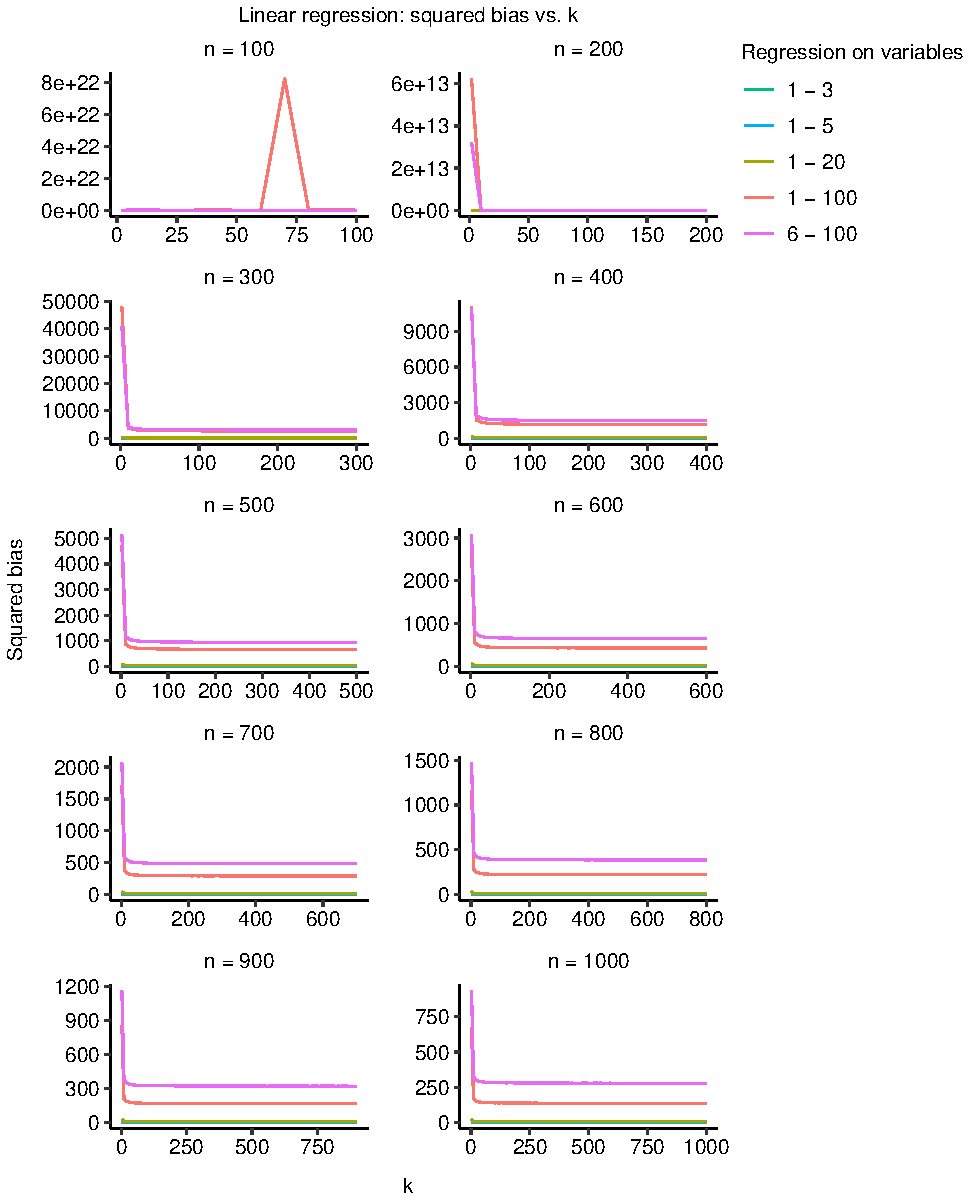
\includegraphics{manuscript_files/figure-latex/unnamed-chunk-1-1} 

}

\caption{Linear regression squared bias vs. fold number for various sample sizes. As fold number increases, bias decreases initially before leveling off.}\label{fig:unnamed-chunk-1}
\end{figure}

\begin{figure}[H]

{\centering 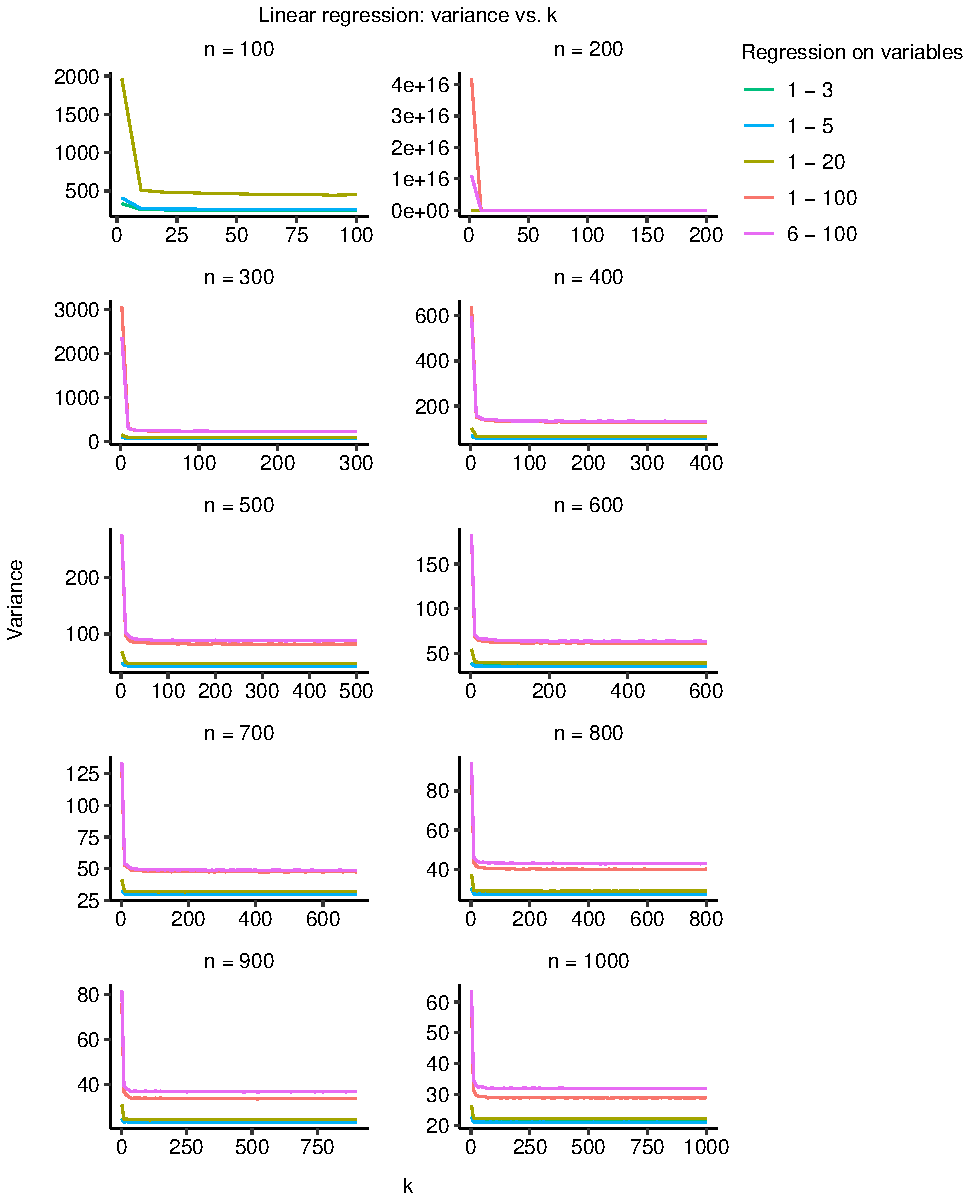
\includegraphics{manuscript_files/figure-latex/unnamed-chunk-2-1} 

}

\caption{Linear regression variance vs. fold number for various sample sizes. As fold number increases, variance decreases initially before leveling off.}\label{fig:unnamed-chunk-2}
\end{figure}

\begin{figure}[H]

{\centering 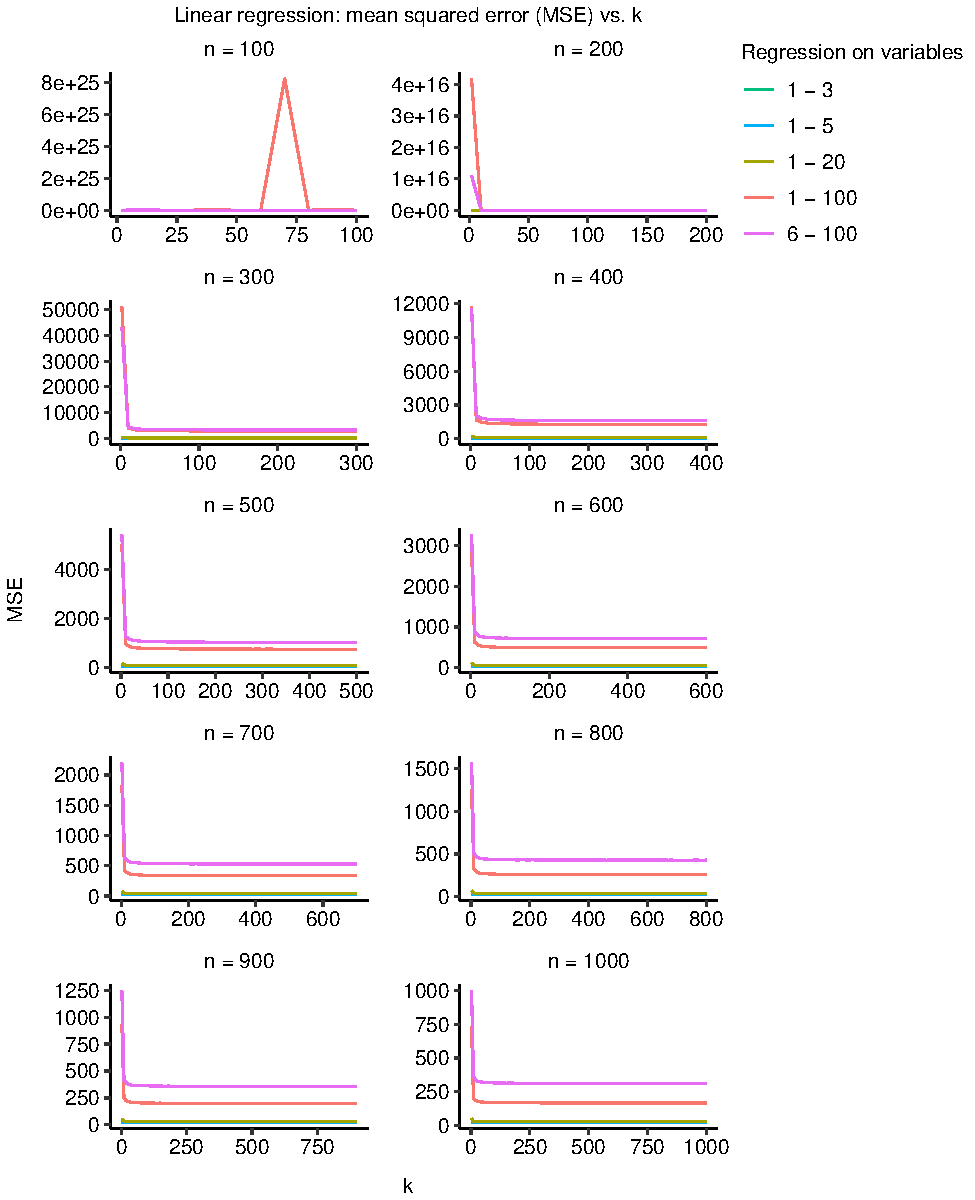
\includegraphics{manuscript_files/figure-latex/unnamed-chunk-3-1} 

}

\caption{Linear regression mean squared error (MSE) vs. fold number for various sample sizes. As fold number increases, MSE decreases initially before leveling off.}\label{fig:unnamed-chunk-3}
\end{figure}

\begin{figure}[H]

{\centering 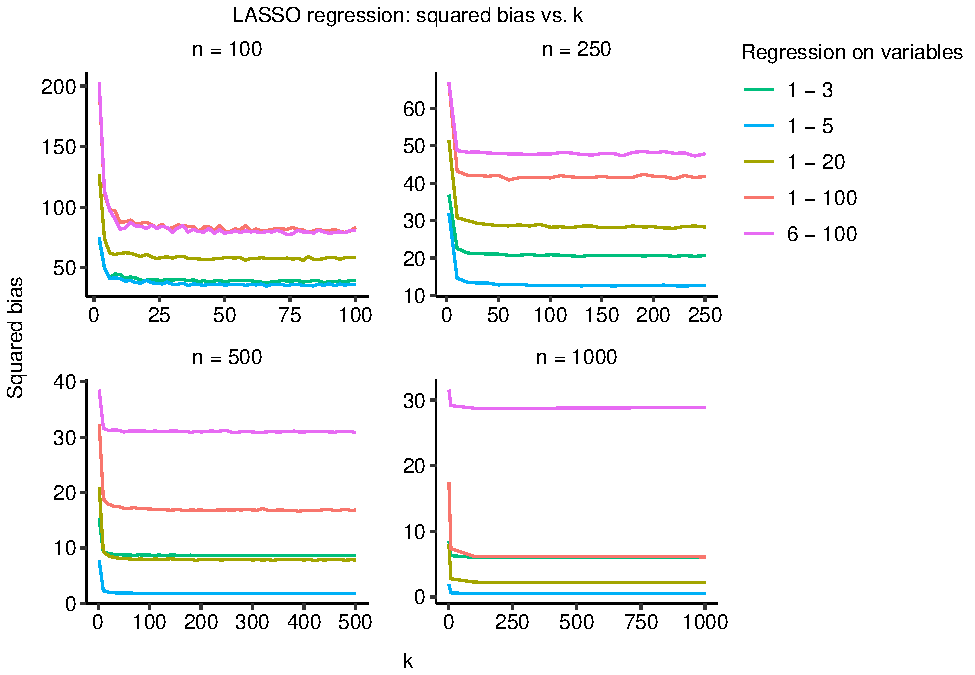
\includegraphics{manuscript_files/figure-latex/unnamed-chunk-4-1} 

}

\caption{LASSO regression squared bias vs. fold number for various sample sizes. As fold number increases, bias decreases initially before leveling off.}\label{fig:unnamed-chunk-4}
\end{figure}

\begin{figure}[H]

{\centering 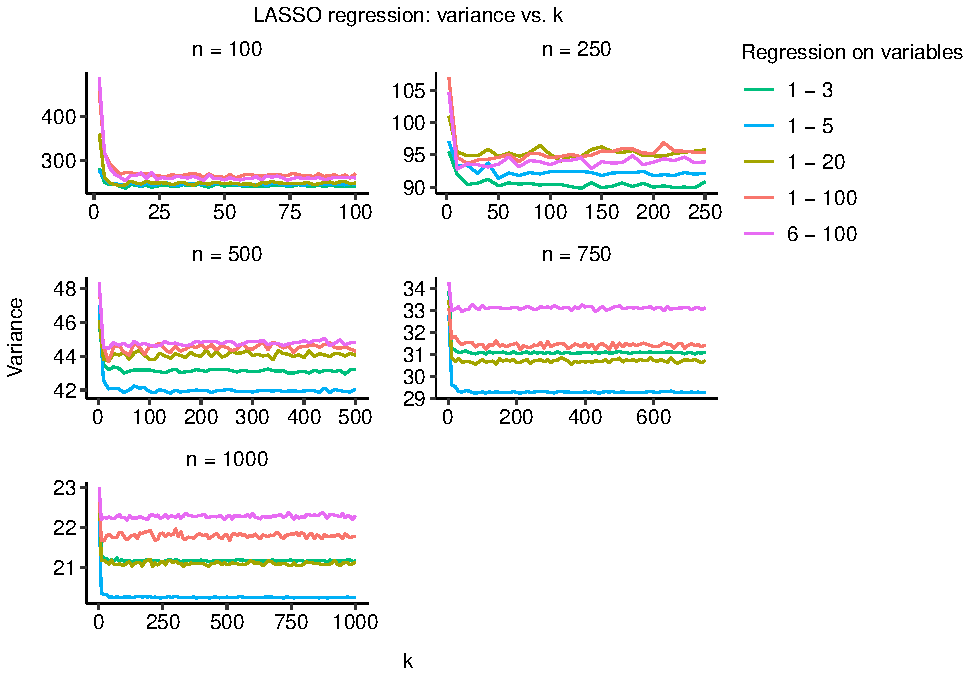
\includegraphics{manuscript_files/figure-latex/unnamed-chunk-5-1} 

}

\caption{LASSO regression variance vs. fold number for various sample sizes. As fold number increases, variance decreases initially before leveling off.}\label{fig:unnamed-chunk-5}
\end{figure}

\begin{figure}[H]

{\centering 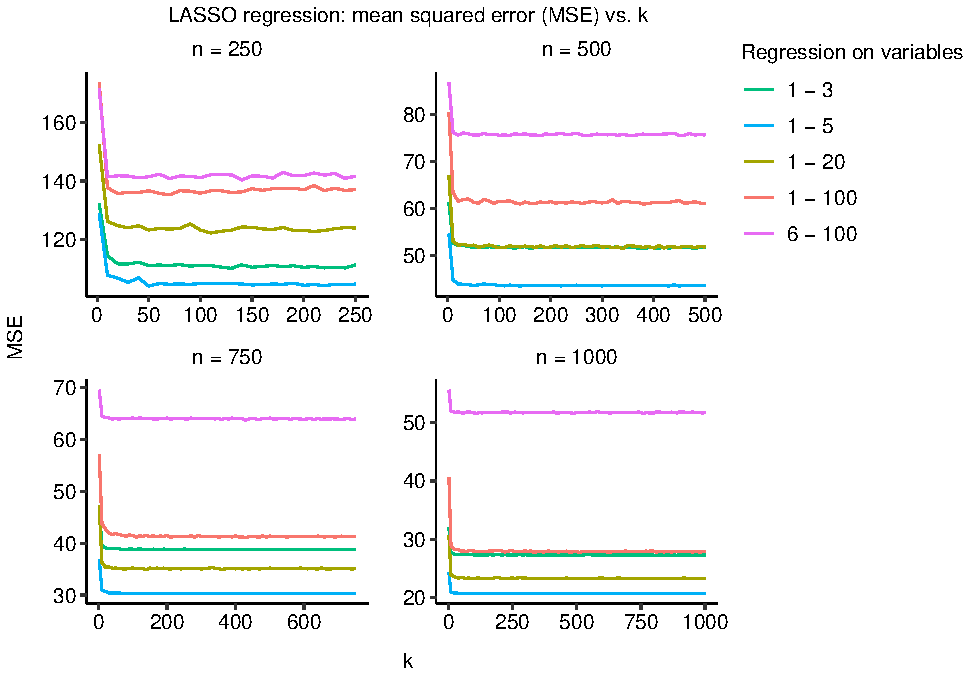
\includegraphics{manuscript_files/figure-latex/unnamed-chunk-6-1} 

}

\caption{LASSO regression mean squared error (MSE) vs. fold number for various sample sizes. As fold number increases, MSE decreases initially before leveling off.}\label{fig:unnamed-chunk-6}
\end{figure}

\begin{figure}[H]

{\centering 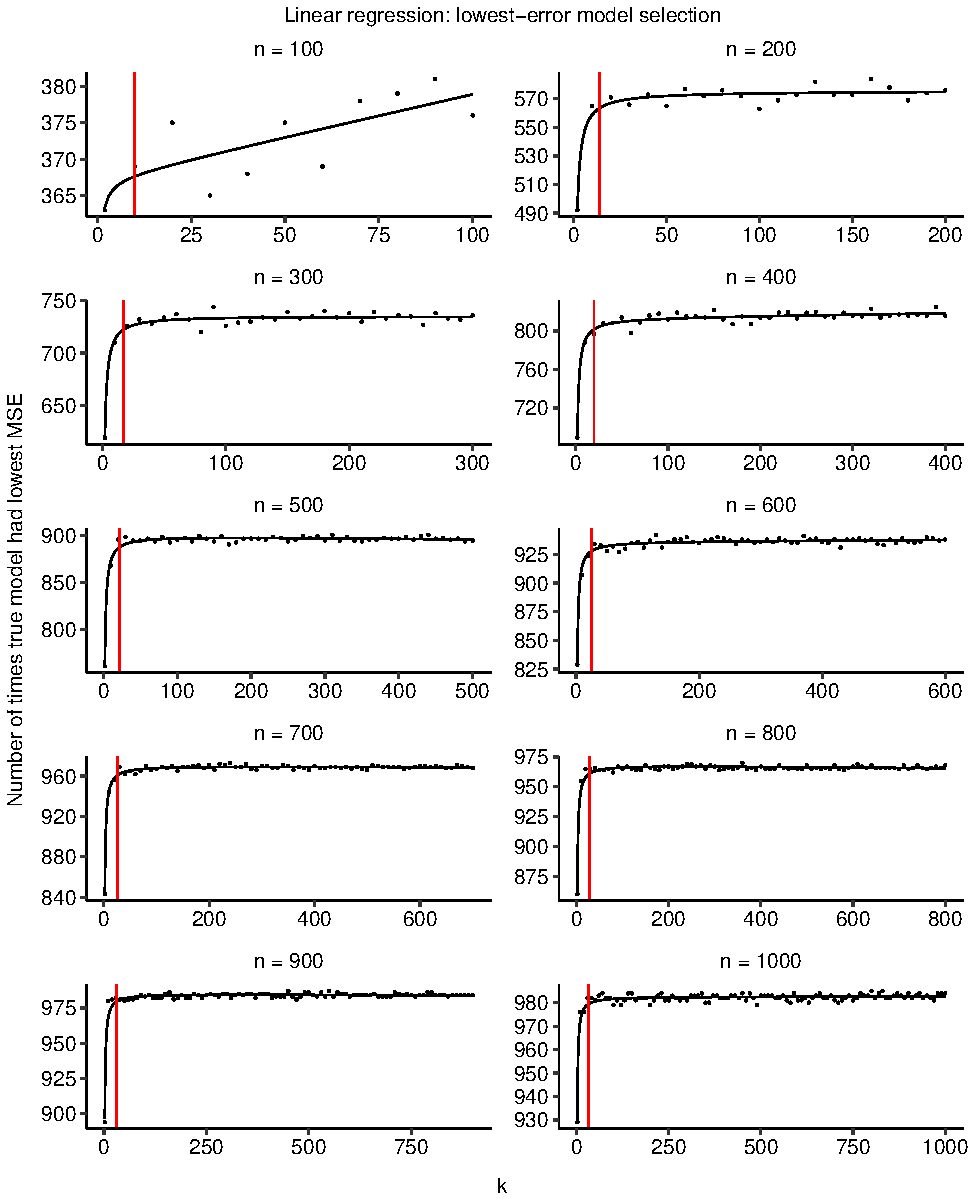
\includegraphics{manuscript_files/figure-latex/unnamed-chunk-7-1} 

}

\caption{Count of true linear regression model selection by the lowest-error criterion vs. fold number for various sample sizes.}\label{fig:unnamed-chunk-7}
\end{figure}

\begin{figure}[H]

{\centering 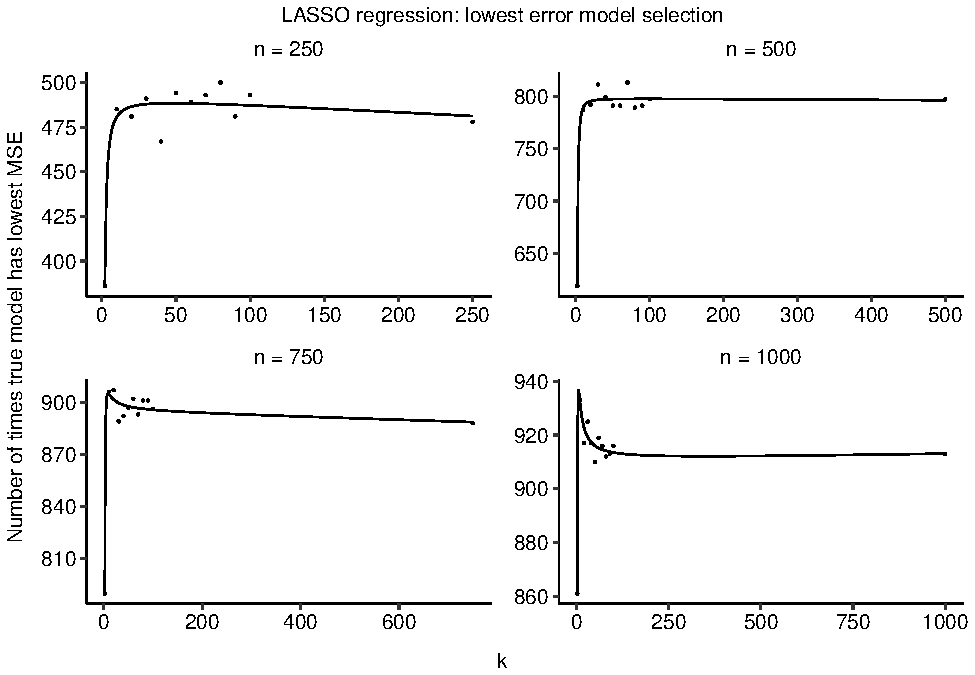
\includegraphics{manuscript_files/figure-latex/unnamed-chunk-8-1} 

}

\caption{Count of true LASSO regression model selection by the lowest-error criterion vs. fold number for various sample sizes.}\label{fig:unnamed-chunk-8}
\end{figure}

\begin{figure}[H]

{\centering 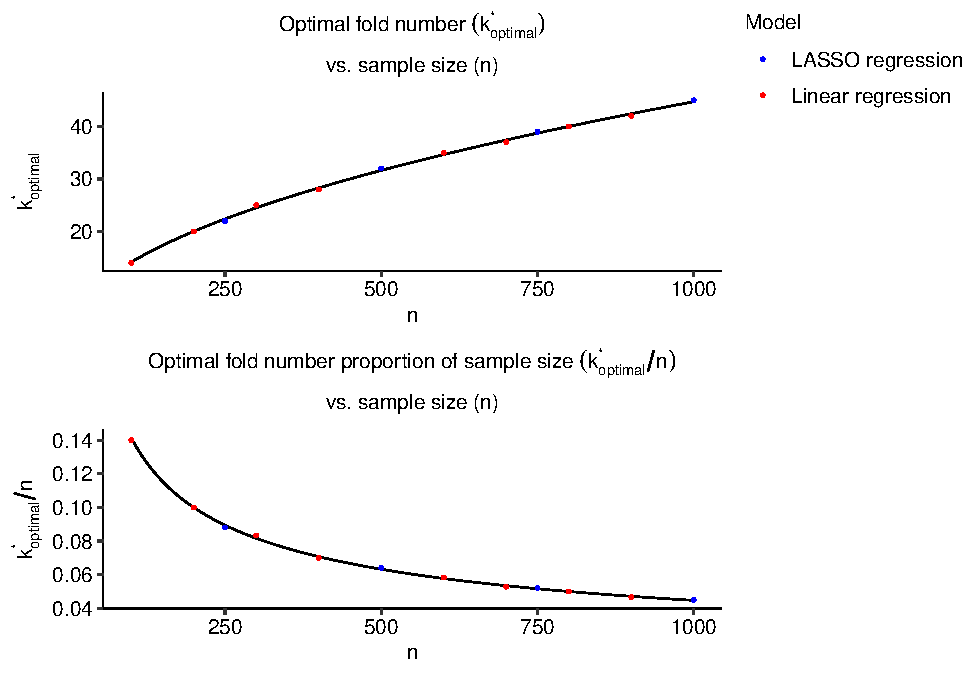
\includegraphics{manuscript_files/figure-latex/unnamed-chunk-9-1} 

}

\caption{Raw optimal fold number vs. sample size (top); fold number proportion of sample size vs. sample size (bottom).}\label{fig:unnamed-chunk-9}
\end{figure}

\hypertarget{acknowledgements}{%
\section*{Acknowledgements}\label{acknowledgements}}
\addcontentsline{toc}{section}{Acknowledgements}

Dr.~Gregory Matthews's Fall 2022 Predictive Analytics class.

\hypertarget{supplementary-material}{%
\section*{Supplementary Material}\label{supplementary-material}}
\addcontentsline{toc}{section}{Supplementary Material}

All code for reproducing the analyses in this paper is publicly
available at \url{https://github.com/gjm112/optimal_k}.

\hypertarget{references}{%
\section*{References}\label{references}}
\addcontentsline{toc}{section}{References}

\hypertarget{refs}{}
\begin{CSLReferences}{1}{0}
\leavevmode\vadjust pre{\hypertarget{ref-Bengio2004}{}}%
Bengio, Yoshua, and Yves Grandvalet. 2004. {``No Unbiased Estimator of
the Variance of k-Fold Cross-Validation.''} \emph{Journal of Machine
Learning Research} 5 (June): 1089--1105.

\leavevmode\vadjust pre{\hypertarget{ref-Breiman1992}{}}%
Breiman, Leo, and Philip Spector. 1992. {``Submodel Selection and
Evaluation in Regression. The x-Random Case.''} \emph{International
Statistical Review / Revue Internationale de Statistique} 60 (December):
291.

\leavevmode\vadjust pre{\hypertarget{ref-Burman1989}{}}%
Burman, Prabir. 1989. {``A Comparative Study of Ordinary
Cross-Validation, v-Fold Cross-Validation and the Repeated
Learning-Testing Methods.''} \emph{Biometrika} 76 (September): 503--14.

\leavevmode\vadjust pre{\hypertarget{ref-Efron1983}{}}%
Efron, Bradley. 1983. {``Estimating the Error Rate of a Prediction Rule:
Improvement on Cross-Validation.''} \emph{Journal of the American
Statistical Association} 78 (March): 316--31.

\leavevmode\vadjust pre{\hypertarget{ref-James2021}{}}%
James, Gareth, Daniela Witten, Trevor Hastie, and Robert Tibshirani.
2021. \emph{An Introduction to Statistical Learning}. 2nd ed. Springer.

\leavevmode\vadjust pre{\hypertarget{ref-Kale2011}{}}%
Kale, Satyen, Ravi Kumar, and Sergei Vassilvitskii. 2011.
{``Cross-Validation and Mean-Square Stability.''} In \emph{International
Conference on Supercomputing}, 487--95.

\leavevmode\vadjust pre{\hypertarget{ref-Kohavi2001}{}}%
Kohavi, Ron. 2001. {``A Study of Cross-Validation and Bootstrap for
Accuracy Estimation and Model Selection.''} \emph{International Joint
Conference on Artificial Intelligence} 14 (March).

\leavevmode\vadjust pre{\hypertarget{ref-Kumar2013}{}}%
Kumar, Ravi, Daniel Lokshtanov, Sergei Vassilvitskii, and Andrea
Vattani. 2013. {``Near-Optimal Bounds for Cross-Validation via Loss
Stability.''} In \emph{Proceedings of the 30th International Conference
on Machine Learning}, 28:27--35. Proceedings of Machine Learning
Research. PMLR.

\leavevmode\vadjust pre{\hypertarget{ref-Marcot2021}{}}%
Marcot, Bruce, and Anca Hanea. 2021. {``What Is an Optimal Value of k in
k-Fold Cross-Validation in Discrete Bayesian Network Analysis?''}
\emph{Computational Statistics} 36 (September): 2009--31.

\leavevmode\vadjust pre{\hypertarget{ref-Yang2006}{}}%
Yang, Yuhong. 2006. {``Comparing Learning Methods for Classification.''}
\emph{Statistica Sinica} 16 (April): 635--57.

\leavevmode\vadjust pre{\hypertarget{ref-Zhang2015}{}}%
Zhang, Yongli, and Yuhong Yang. 2015. {``Cross-Validation for Selecting
a Model Selection Procedure.''} \emph{Journal of Econometrics} 187
(February): 95--112.

\end{CSLReferences}

\end{document}
